Lung cancer symptoms may vary depending on the type, stage, and location of the cancer. Common symptoms include:

\begin{highlight}
\begin{itemize}
    \item Persistent cough that does not go away or worsens over time.
    \item Coughing up blood (\textcolor{red}{hemoptysis}) or rust-colored \textcolor{red}{sputum}.
    \item Shortness of breath (\textcolor{red}{dyspnea}).
    \item Chest pain or discomfort, especially when breathing deeply, coughing, or laughing.
    \item \textcolor{red}{Hoarseness} or changes in voice.
    \item Unexplained weight loss or loss of appetite.
    \item \textcolor{red}{Fatigue} or feeling weak.
    \item Frequent infections, such as \textcolor{red}{bronchitis} or \textcolor{red}{pneumonia} .
    \item \textcolor{red}{Wheezing} or noisy breathing.
    \item \textcolor{red}{Swelling} in the face, neck, or upper body (\textcolor{red}{superior vena cava syndrome}).
    \item Bone pain or \textcolor{red}{tenderness} (if cancer has spread to bones).
    \item \textcolor{red}{Neurological symptoms}, such as headache, dizziness, or numbness, if the cancer has spread to the brain.
\end{itemize}
\end{highlight}
\begin{remark}
Note that many of these symptoms can also be caused by other conditions. It is important to consult a healthcare provider for an accurate diagnosis.
\end{remark}
\begin{figure}[h!]
    \centering
    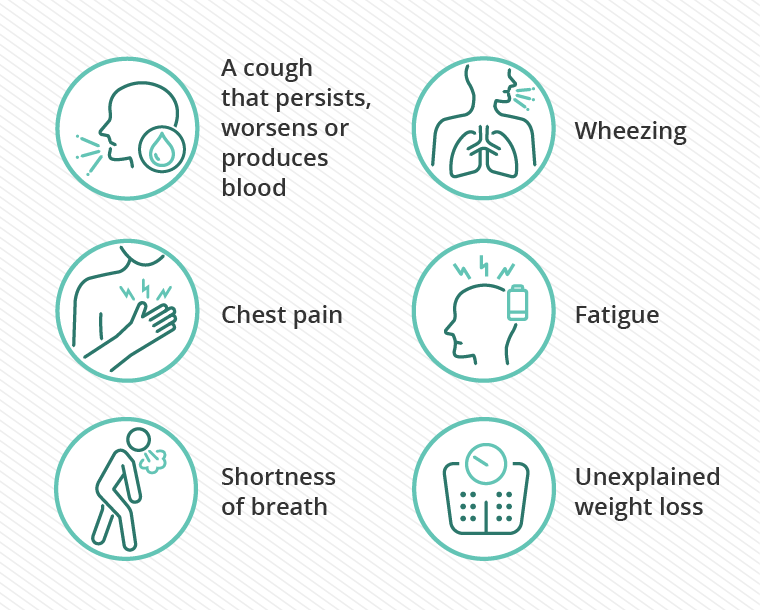
\includegraphics[width= 0.675\linewidth]{images/Lung-Cancer-Symptoms-DT.png}
    \caption{Symptoms of lung cancer}
    \label{fig:symptoms}
\end{figure}

\newpage